\chapter{Simulated Illumination and Tension in Games}
As established earlier, the lighting of a given scene can greatly define the atmosphere in a game. However, to discuss some lighting techniques and rules, one first has to define the vocabulary that is used to describe the behavior of light in a video game.

\section{Translating from reality to games}

Simulated illumination is defined as the method by which virtual (3D) game environments are rendered taking into account all lighting information in the scene.\cite{Maggi.2006} Of cause, the style of these simulations are not set in stone and can range, depending on the capability's of the game engine and the artist's vision, from very stylized to nearly photo-realistic. In an effort to define such vocabulary for the lighting of a scene, light designer Louis Clair first laid out some characteristics of lighting in the real space.\cite{Niedenthal1404353}:

\begin{enumerate}
    \item \textbf{Brightness or luminance} \\
    In the real world, this can be measured in lux or lumens. This depends, whether the light is measured at the receiving surface(lux) or at the source (lumen) \cite{LuxAndLumens}
    \item\textbf{Color} \\
    Can be expressed through the color rendering index \cite{colorrendering}, measured through degrees Kelvin, specified through chromatic diagrams or even verbal descriptions
    \item \textbf{Direction, distribution, and movement from the source} \\
    This can be indicated with a system of arrows or with a lighting distribution diagram \cite{dmlights}
    \item \textbf{Shadow quality}\\
    The density and quality of hard or soft shadows and their edges.
    \item \textbf{Contrasts}\\
    The Contrast between different layers in a given room.
\end{enumerate}



While not all these measures are relevant or even possible to implement in digital lighting simulations \cite{Niedenthal1404353}, all of them can be taken into account by a lighting artist for virtual environments in modern engines. 

Using the above characteristics, the color of a given light, for example, can be specified by an RGB-Value. The direction and distribution can be set by using different forms or combinations of light emitters such as point lights, spotlights and directional (parallel) lights. Spatial contribution, speed or luminance can be accessed through the games code and contrasts can be, if not generated to the artist's liking, be manipulated by post-processing effects. 
\newpage
For designing such a light simulation (or any other simulation for that matter), one has to make choices, which define the arrangement, setting and configuration of lights in a virtual Scene. Therefore, Simon Niedenthal describes four key steps of the process of developing such a simulation\cite{Niedenthal1404353}: 

\begin{enumerate}
    \item Acquisition of source information about the subject
    \item Selection of key characteristics and behaviors of the subject
    \item The use of simplification, approximations and assumption within the simulation
    \item Fidelity and validity of the simulation outcome has to be confirmed
\end{enumerate}

By executing, and therefore implementing, these steps, it becomes obvious, how lighting algorithms have evolved over time. The Step of acquiring information about a given scene dates back even to the 9th century. Ranging from Arab philosopher Al. Hazan (specular reflections) over Newton, who formulated the inverse square law used to calculate the falloff of light intensity to Lambert (1760) (diffuse reflections). \cite{Niedenthal1404353}. 

Complex characteristics (2) of lighting are developed in relatively recent years. An early example of such, more complex, technique is  color bleed, which first has been rendered by Goral et al. in 1984 \cite{Goral84} 

The complexity of light simulations, even when kept relatively simple, has introduced a tight performance budget and therefore many simplifying algorithms (3) had to be used to ensure a reasonable framerate for real-time simulations. Early lighting algorithms focused on the recreation of direct light effects and didn't take more complex shading and indirect lights into account \cite{Niedenthal1404353}, Historically, this tight budget of processing introduced by the complexity of a lighting simulation has drastically limited the number of light sources and fidelity of effects that could be used in a scene for a real-time simulation of light (aka. video a game). Only in recent years, the capability of real-time engines and computer hardware had created enough headroom to loosen the performance budget a bit and create more variant graphical effects and lighting techniques \cite{Niedenthal1404353}. An example of this is the rise of real-time ray tracing, which was first implemented by Nvidia and then also by AMD for real-time graphics. This allows for the simulation of indirect light and global ambient occlusion with a relatively low tax on the performance budget \cite{RTXON}. This, in turn, has significantly increased artistic freedom and enabled more versatile and elaborate levels. 

The validation step (4) is, in many cases, the hardest to execute, since video games are, more often than not, creating a space, which does not exist in real life. However, Goral, for example, validated his algorithm for color bleeding by comparing his computer-generated render and its RGB values at certain places with a real-life representation of the same scene. The real-life color values were taken with photometric readings. \cite{Goral84}. In the case of computer games, this step of validation is also often a play test, in which it is asked whether the player experiences the desired emotion and whether the desired atmosphere is created. 
\newpage
\section{Using simulated illumination as a design material}

Light and therefore design of lighting effects has long been seen as the basis of our perception of space and form. This is true for many media besides video games such as film, theater or computer animation. In recent years, especially with the ever-lasting rise of processing power and capability of lighting algorithms light has been used to convey a deeper design aspect: Light can be used to manipulate, how a player sees a scene and how he reacts to it. It can manipulate feelings and has a deep connection to the player's emotions. Moreover, it can be used to create a more believable and dramatic environment for the player to immerse himself in. Therefore creating a much deeper and defined atmosphere. \cite{Shadowplay}
\\\\
The creation of such immersive and visually rich lighting setups for game environments leaves the game developer with a great deal of artistic freedom. Unlike in other lighting design tasks (as for example in architecture or theater), game lighting has to be created entirely from scratch. Every surface, form and character has to be considered and has to blend in the rest of the scene. Given these differences, a light designer might be tempted to only focus on the end result (the rendered frame) and disregard the spatial relations and placements of each light source. However, due to the dynamic nature of video games, the player can alter his position in a scene, which leads to a completely different lighting situation, which the lighting designer also has to take care of. \cite{Niedenthal1404353}
\\\\
Currently, lighting practices for the creation of 3D environments in video games, are heavily inspired by traditional media such as animation, film, theater and even architecture. This is, in part, due to the lack of specific research on game lighting and interactive scenes \cite{Maggi.2006} and the similarities, which are existent between the design of a traditional, static, scene and an interactive scene in a video game: A light designer of an interactive scene still has to stage lights in a three-dimensional environment, identify attributes such as color, intensity, spacial contribution and shadows and thereby setting the desired atmosphere of a virtual scene.
\newline
To define the goals of a lighting setup in virtual scenes, Sharon Callahan, a lighting designer at Pixar proposed five design goals for creating a synthetic scene\cite{Storytelling}: 
\begin{enumerate}
    \item Directing the viewer's eye
    \item Creating depth
    \item Conveying time of day and season
    \item Enhancing mood, atmosphere and drama
    \item Revealing character personality and situation
\end{enumerate}
\newpage
So as seen, the process of designing a lighting setup for interactive media contains two elements: At first it is descriptive for the user. It helps him to "make sense of the scene". It accomplishes that by highlighting important items, guiding his way to the next passage to progress in a story or a task or simply adding readability to his surroundings. 
The other element, and focus of this seminar report, is to convey a deeper meaning. Lighting can be (and is) directed towards the players emotion and understanding of narrative structures. These five design goals all support components of a players experience in a video game: attentiveness, absorption,
coherence, emotion and "make-believe",\cite{Niedenthal1404353} thus creating a game's atmosphere. 
Those design goals largely reflect Pixar's influence on lighting research in virtual scenes. In a video game, however, the player can take as much time as he wants to experience, manipulate and investigate the lights in a scene and the work that went into it\cite{Maggi.2006}. Thus it opens up the opportunity to explore the emotional content of designing lights in interactive media. 

\section{Designing the lighting simulation}
\subsection{Drawing upon experience from other media}
In his book "The Language of New Media" from the year 2000, Lev Manovich states, that "the visual culture of the computer era is cinematographic in appearance". This, for the most part, still holds true. As established above, game creators use a filmic vocabulary when creating a lighting arrangement in virtual scenes. Game elements such as cut scenes clearly suggest the use of these, already established, therms. Moreover, certain larger lighting strategies such as face lighting conventions, time of day, narrative elements and mood translate really well to the filmic approach \cite{Shadowplay}. Obviously, however, many elements of game lighting can not be transferred to the filmic approach. Traditional media, animated or in life-action, are from a fixed perspective and the light is directed to this one perspective. Games however are an interactive medium and allow the player to explore the scene from many different angles and different timeframes \cite{Maggi.2006}. Thereby, it makes sense to compare the process of designing lighting in a game to the work of an architectural lighting designer. Grodal even points out, that video games evoke first-person emotions rather than third-person emotions. Accordingly to him, this happens because games implement some motion controls to interact with the player and thus simulate real-world patterns of interactions \cite{Grodal}. 
\newpage
\subsection{Drawing upon experience of real spaces}
Brenda Laurel said in her work "Computers as Theater", that we always take a subset of our senses with us, when we engage in virtual environments. Following this argumentation, it can be claimed, that virtual experiences, at least in part, can be translated to our real-world experience, when exposed to a carefully set up light scene. Of cause the player's experience, when confronted with a virtual scene can not directly be translated into a real-world experience. Virtual experiences are  (in most cases) transmitted through a flat-screen occupying only a portion of our field of view and having limited space of colors whits intern limits the range of the simulated illumination. \cite{Niedenthal1404353}. Nevertheless, according to Gibsen, our encounter with light, even in a virtual environment, still triggers a direct response to its light; “a picture,” he writes, “is a surface so treated that (it) contains the same kind of information that is found in the ambient optic arrays of an ordinary environment” \cite{Gibson71}.
If we accept this and see simulated illumination as related to real illumination and its triggered reaction, we can benefit off of many types of research, that have been conducted for real-life lighting and its effects on the human. Many (though obviously not all) can be reused for information on how to light virtual scenes. Much research in the past tries to establish a standard of how much and which light best supports intense visual tasks in work and public spaces \cite{Niedenthal1404353}. An additional example is Kenz, who researched during his study conducted in 2001 the effects of not directly visible illumination upon the emotion of a subject \cite{Knez2001}. Knez even has proposed a link between the temperature of lighting (red and blue) and the mood of a player and discovered different emotional reactions to these temperatures of color. These finding's indeed not only introduce a new approach to the study of visual effects and their simulation. It also opens up new potential for designing the lighting in a game to trigger certain physical responses which help the player to immerse himself in the scene. 
\newpage
\subsection{Designing lighting in a video game}
\label{chap:witcher}
When looking at video games and their lighting it becomes obvious, that we can not only rely on experience made in the real world and research from other forms of media. To elaborate this, "The Witcher 3" from the polish company CD Project RED is taken as an example. This game gives the player the mechanic to toggle an ability to view extra hints, clues and objects in the game world. This is conveyed by an overlay (see Figure \ref{fig:witcher}), which is not orientated by any traditional forms of light design or visual effects. \cite{witchersenses}

\begin{figure}[h]
	\centering
		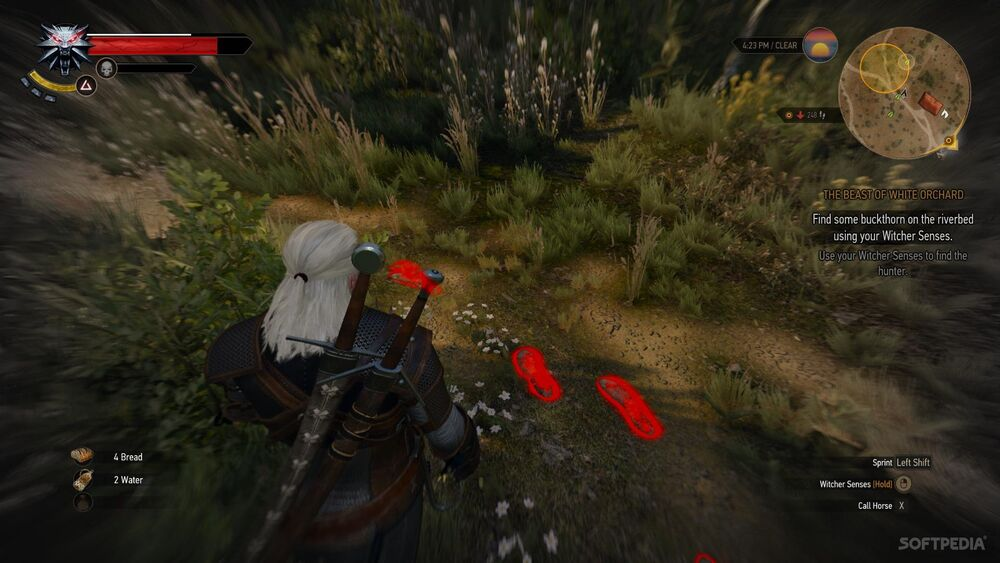
\includegraphics[width=0.9\textwidth]{Bilder/The-Witcher-3-Diary-Witcher-Contracts-Are-Quite-Fun-482236-2.jpg}
	\caption{The "Witcher Sense" in the game The Witcher 3 \cite{witchersenses}}
	\label{fig:witcher}
\end{figure}

It gives the player the possibility to visualize objects in the game scene, that are are not visible using common means of visible light. These include highlights of objects and tracks, that are important clues to solve a puzzle, the player is confronted with. These visual effects can also mark enemies or other dangerous entities. This lets the player, with the press of a button, completely change the visual appearance of the game. In this case, it is even an unnatural, not found in any real observations or literature, style. Another example of a specific challenge of light design, which is only applicable to games and other forms of interactive media is the active manipulation of light by the player. For example, Flashlights can drastically alter the mood and the player experience of the player within a virtual scene and the way the player interacts with a given scene \cite{Shadowplay}.
\newpage
In summary, the interactive nature of a video game both widens the designer's possibilities to create rich and compelling atmospheres but also imposes new concerns and design guidelines that have to be taken care of. Simon Niedenthal, therefore, laid out 3 considerations for a lighting designer working on interactive virtual scenes to be made \cite{Shadowplay}: 

\begin{enumerate}
    \item \textbf{Defining the basic characteristics of the illumination of the environment in time and space}\\
    Even if the player might has the ability to alter the lighting of a virtual scene by adding light (e.g. with a flashlight or car headlights) or subtracting light (e.g. by shooting out lights or blocking sources of light), the designer has to create a base lighting for his scene. This can consist of a base ambient lighting, essential shadows and their density and quality, or outlining the visual features of the world. Here he can apply some techniques used in film and other static types of media such as "high-key" or "low-key" (elaboreted in section \ref{cap:highLow}) strategies. High-key traditionally is associated with comedy and lighter fare whereas low key is most commonly associated with horror, survival and more dramatic scenes. 
    
    \item \textbf{Outlining the capabilities of the player}\\
    As described above, in the game "The Witcher 3" the game scene can be drastically altered by the abilities of the player and therefore presented in a whole different visual style. Offering the player a set of choices, which are communicated through the use of visual effects and lighting. In this case, it conveys a sense of mastery over the environment and other characters within the game. Other examples however can also convey a sense of vulnerability: In the Game "Splinter Cell" the player's flashlight can uncover important entities within the game world, but can also alert enemies.
    
    \item \textbf{Integrating illumination concerns within the game's experience}\\
    The lighting artist has to integrate the lighting in the feel of the game. The visual effects have to harmonize with other aspects of the game's design (for example sound). This step also includes making player actions meaningful and to create a coherent experience for the game as a whole and therefore creating a believable and dense atmosphere. 
    
\end{enumerate}
\newpage
\section{The influence of virtual lighting on game worlds} \label{cap:simu}

To describe a simulation of light as good as possible, one can say, that it "visually describes game environments and brings them out of formlessness" \cite{Niedenthal1404353}. However, as already established in early sections of this work, digital lighting in video games opens up much more potential and enables the game's designer to convey higher-level emotions and atmospheres to the player. In his work "Complicated shadows: The aesthetic significance of simulated illumination in digital games" Simon Niedenthal proposes six design influences that have a direct impact on the player's experience of a game and thus its atmosphere. These will be elaborated within the following chapter and ordered. Each will have a greater impact on the player's sense of atmosphere than the last. 

\begin{enumerate}
    \item \textbf{Exposure} (direct experience of light qualities in virtual environments) \\
    As established in early chapters, specific illumination patterns have the ability to influence our subconscious feelings. "When we are exposed over a period of time to light, qualities such as brightness or color have the ability to affect our emotions and behavior. This occurs through activation (how aroused we become), as well as affect, or mood (Knez 2001)\cite{Knez2001}" That means, when specific lighting combinations predominate in virtual, interactive, environments, we can expect certain contributions to the players affection mood and atmosphere \cite{Shadowplay}.

    \item \textbf{Contrast} (variations of light qualities within the visual field)\\ 
    It is unlikely that the player will be confronted with a scene that has only one source of illumination or is homogeneously lit. Most of the scenes the player will be confronted with are built from a variety of elements, such as different light colors, natural and artificial light, shadows and etc. Our perception of contrasts, which are expressed through light differences in the scene, is one of the main mechanisms by which scenes are perceived and understood. For example, as mentioned earlier in Callahan's design goals, contrast is one of the main ways in which the player's attention can be drawn.  \cite{Storytelling}
    
    \item \textbf{Temporal change} (as a function of player navigation from environment to environment, as well as external influences) \\
    Many light effects and elements are perceived by the player only through a temporal shift. The design language is only revealed when the player moves through a level or waits for some time. Examples include the difference between day and night, light and dark, and warm and cold. Longer-term lighting changes can also be used as a stylistic device in games, for example, to convey progress or the story. By holding back or highlighting some lighting changes, the player's emotional experience is also pushed further. Generating a denser atmosphere. \cite{Niedenthal1404353}
    
    \item \textbf{Lighting patterns and conventions} (recognition of illumination patterns from other games and media types, genres, characters, etc) \\
    A closer look at the transfer of a lighting atmosphere from the real world to the virtual one quickly reveals a number of procedures from other media and games. These occurrences describe an impression that we associate with the atmosphere of a certain genre or the emotions of a certain image. As Callahan noted, these lighting and visual effects have the potential to illustrate the character and personality of a figure or even a scene. Thus they contain important tools and techniques to properly design the visuals of a game \cite{Storytelling}
    
    \item \textbf{Lighting effects} (moments at which the player becomes aware of light qualities, either to enhance the immediate game environment or to engage Atmosphere)\\
    In video games, there are often individual moments in which visual effects become particularly obvious. These effects are often used, for example, to draw attention to certain parts of the environment. This is the case, for example, with the so-called "godrays", which showcase the impact of light in a weaker lit part of the scene. Light effects can also be assigned a metaphorical function, for example in the game "Shadow of the Colossus", in which a light shine emanates from talking characters. \cite{Niedenthal1404353}
    
    \item \textbf{Interaction and player agency} (strategic or tactical player activity related to lighting, or lighting that serves as a feedback device for player action)\\
    Quite often, a player is not simply confronted with predetermined lighting, but can actively help shape it. For example, as seen in the example of the "Witcher senses" in "The Wither 3" (see Figure \ref{fig:witcher}), a supernatural ability can be illustrated, which gives the player a feeling of superiority. Lighting can also be used tactically, as in the case of Splinter Cell: In this stealth game, lights are shot out to further envelop the player in protective darkness. 
    
\end{enumerate}

The methods described above give the artist a variety of tools to enhance and develop the aesthetics and the atmosphere as well as the involvement of the player.